\reportheading{2. DIALux modelling and simulation}

\subhead{2.1 Geometry and manufacturer photometry}

The architectural drawing imported into DIALux evo was verified against the 45 m overall dimension to reduce scale mismatches. Following this, to account for light obstruction, the office boundary and eight full-height columns were modelled.

Moreover, the light distribution data from the manufacturer's ULD file is used in the calculation [3], while DIALux calculates reflected light using the surface reflectances listed in Table 1. The fittings sit within the 600 mm ceiling tiles and have their light-emitting faces aligned with the 2.8 m ceiling, whereas in the DIALux simulation report, the luminaire reference position is listed at 2.868 m, which is 68 mm above the ceiling plane. Figure 1 depicts the model alongside the evaluation heights.

\reportfigure{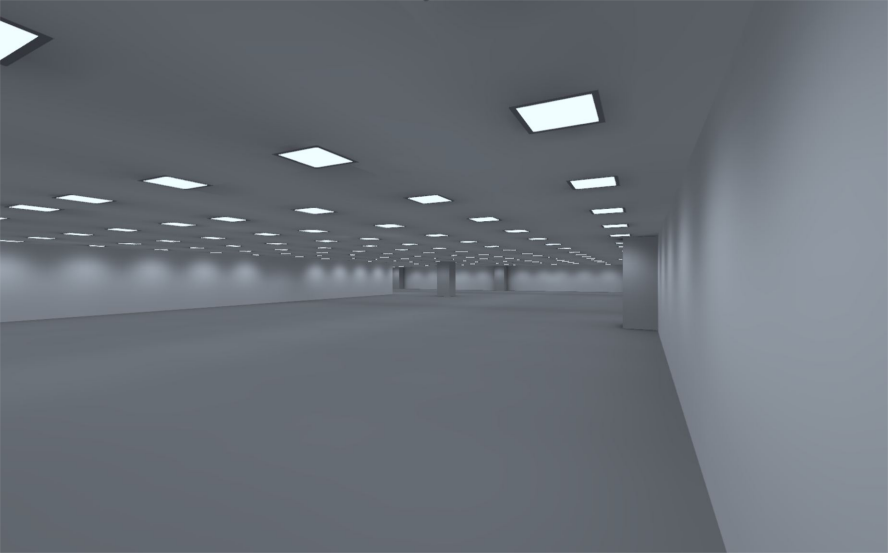
\includegraphics[width=.45\linewidth]{../Assets/native-room-view.png}\hfill\includegraphics[width=.47\linewidth]{heights.pdf}}{Figure 1. Native room view (left) and adopted calculation heights (right).}

\subhead{2.2 Task-area calculation}

Each 1.6 by 0.8 m desk has a 10 by 5 calculation grid at 0.8 m height. According to EN 12464-1 clause 5.4, a 2:1 area is governed by its short side, which limits the maximum spacing to 0.2 × \(5^{\log_{10}(0.8)}\) = 0.171 m [1]. As a result, the selected 0.16 m grid meets this requirement. Meanwhile, DIALux defines the overall uniformity \(U_{\mathrm{o}}\) as the ratio of minimum to mean illuminance [4]. Ultimately, individual desk checks are essential to prevent some poorly lit workstations from being overlooked due to a satisfactory room average.

\subhead{2.3 Maintenance factor and glare}

By applying a maintenance factor of 0.80, the gradual reduction in illumination is accounted for over time [5]. In addition, glare was calculated at a seated eye height of 1.2 m across viewing directions at 15-degree intervals [6]. While the manufacturer gives a catalogue UGR value for the fitting, the glare experienced in the office also depends on luminaire positioning and office surroundings, therefore, the calculated room values are compared against the UGR limit.

Furthermore, calculations were applied to the 0.5 m bands around the bench groups, the remaining background floor, cylindrical illuminance at seated head height, and the exposed walls and ceiling. The same fittings and positions were maintained for the desk calculation, where the desks serve as calculation surfaces, whereas solid furniture, monitor screens, and high partitions are excluded. Finally, separate copies were used for the output and reflectance comparisons, with all other inputs held constant.
